\documentclass{jarticle}

% 画像
\usepackage[dvipdfmx]{graphicx}
% リンク
\usepackage[dvipdfmx]{hyperref}
% URL
\usepackage{url}
% 目次
\usepackage{pxjahyper}
% フォント関連
\usepackage{amsfonts}
\usepackage{amsmath, amssymb}
\usepackage{mathrsfs}	% for \mathscr{}
\usepackage{bm}
\usepackage{here}
\usepackage[super]{cite}
% ソースコード表示のための設定
\usepackage{listings,jlisting}

\renewcommand\citeform[1]{[#1]}

\lstset{
  basicstyle={\ttfamily},
  identifierstyle={\small},
  commentstyle={\smallitshape},
  keywordstyle={\small\bfseries},
  ndkeywordstyle={\small},
  stringstyle={\small\ttfamily},
  frame={tb},
  breaklines=true,
  columns=[l]{fullflexible},
  numbers=left,
  xrightmargin=0zw,
  xleftmargin=3zw,
  numberstyle={\scriptsize},
  stepnumber=1,
  numbersep=1zw,
  lineskip=-0.5ex
}

% 余白の設定
\usepackage[margin=20truemm]{geometry}

\begin{document}
\title{1年生実習 第2週}
\author{B5研究室}
\date{2024年6月26日}
\maketitle

\section{実習概要の変更}

先週配布した資料に記載のスケジュールから,大きく変更があります.

\begin{description}
  \item[第1週] Python入門
  \item[第2週] Leap Motionによるデータ取得 \& テクニカルライティング
  \item[第3週] 機械学習によるデータ分類
  \item[第4週] プレゼンテーションテーマの決定
  \item[第5週] プレゼンテーション作成と練習
  \item[第6週] プレゼンテーション本番
\end{description}

\section{機械学習とは}
機械学習とは,人工知能の一分野であり,データからパターンを発見し,そのパターンを利用して未知のデータに対する予測を行う技術です.
今週と来週の実習では,機械学習について深く踏み込むことはせず,実際にデータを取得し,
機械学習を用いてデータを分類するというプロセスを体験することに重点を置いています.

\subsection{機械学習のプロセス}
機械学習のプロセスは,以下のようになります.
\begin{enumerate}
  \item データ取得
  \item データ前処理
  \item モデル構築
  \item モデル評価
  \item モデル改良
\end{enumerate}



\subsection{データ取得}
データ取得とは,センサーやデバイスを用いて,様々な情報を取得することです.
データ取得を行うことで,様々な情報を取得し,それを解析することで,新たな知見を得ることができます.

\subsection{データ前処理}
データ前処理とは,取得したデータを整形し,機械学習アルゴリズムに適した形に変換することです.
データ前処理を行うことで,機械学習アルゴリズムの精度を向上させることができます.
データ前処理によって,モデルの性能が大きく変わることもあるため,重要なステップといえます.
データ前処理手法の例としては,次のようなものがあります.

\begin{itemize}
  \item 欠損値の補完
  \item カテゴリ変数のエンコーディング
  \item 標準化
  \item 正規化
\end{itemize}

各手法の説明については,割愛しますが,興味のある方は,機械学習の入門書などを参考にしてください.

\subsection{モデル構築}
モデル構築とは,データを用いて,機械学習アルゴリズムを用いてモデルを構築することです.
モデルとは,データからパターンを発見し,未知のデータに対する予測を行うための数学的なモデルのことです.
具体的には,実際にデータを入力して,目的のタスクを行う部分です.
論文等で効果が検証されているモデルを使用することが多いですが,タスクによっては,自分でモデルを設計することもあります.

\subsection{モデル評価}
モデル評価とは,構築したモデルの性能を評価することです.
モデル評価を行うことで,モデルの性能を把握し,モデルの改良を行うための方針を立てることができます.
モデル評価は,モデル構築と同様に重要なステップであり,慎重に行う必要があります.
モデル評価には,様々な指標がありますが,代表的なものとして,以下のものがあります.
\begin{itemize}
  \item 正解率
  \item 適合率
  \item 再現率
  \item F値
  \item ROC曲線
  \item AUC
\end{itemize}

\subsection{モデル改良}
モデル改良とは,モデルの性能を向上させるために,モデルの構造やパラメータを調整することです.
モデル改良を行うことで,モデルの性能を向上させることができます.
モデル改良には,ハイパーパラメータの調整や,特徴量の追加などがあります.
モデル改良は,モデル評価の結果をもとに行うため,モデル評価が重要なステップであることがわかります.

\section{Leap Motionによるデータ取得}
本実習では,Leap Motionを用いて,空中入力による手書き文字データを取得します.
本研究室には,Leap Motionを実際に研究で使用している人もいます.
2年次のソフトウェア設計および実験では,希望すればゲーム制作に使用できる(ハズ)です.

\subsection{Leap Motionとは}
Leap Motionは,赤外線を使用した,ジェスチャー認識を行うためのデバイスです.(図\ref{fig:leapmotion})
Leap Motionを用いることで,手の動きを検出し,その情報を取得することができます.
今回の実習では,各自のPCに環境構築はせず,研究室内のPCを使用して空中入力による手書き文字データを取得します.

\begin{figure}[H]
  \centering
  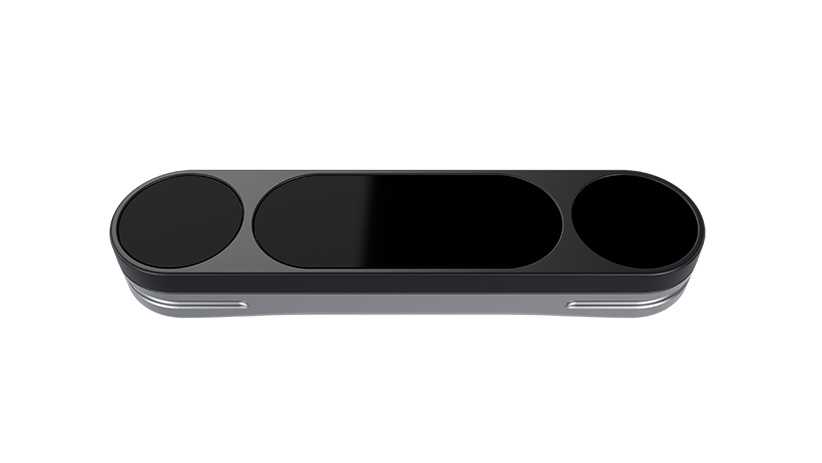
\includegraphics[width=10cm]{fig/leapmotion.png}
  \caption{Leap Motion \cite{leapmotion} (画像は第2世代)}
  \label{fig:leapmotion}
\end{figure}

\subsection{データ取得手順}
データ取得の概要を表\ref{table:data_acquisition}に示します.
\begin{table}[H]
  \centering
  \caption{データ取得の概要}
  \begin{tabular}[H]{c|c } \hline
    \label{table:data_acquisition}
    項目 & 内容 \\ \hline
    取得文字 & $ \bigcirc  \times $ の2文字\\
    取得文字数 & 3セット $ \times $ 11人の66文字 \\ \hline
  \end{tabular}
\end{table}

\section{テクニカルライティング}
テクニカルライティングとは,技術文書を書くための技術のことです.
技術文書とは,技術に関する情報を伝えるための文書のことであり,論文や報告書,マニュアルなどがあります.
技術文書を書く際には,読み手に正確に情報を伝えることが求められます.

時間の都合上,ここではテクニカルライティングの基本的な部分のみを説明します.
テクニカルライティングには,以下のようなポイントがあります.
\begin{itemize}
  \item 要点を明確にする
  \item 短くまとめる
  \item 正確な情報を伝える
  \item 読み手に合わせて書く
  \item 1文で伝えることは1つのみにする
\end{itemize}

以上の項目を意識して報告書を書くことで,読み手に正確に情報を伝えることができます.

逆に,読み手が書き手の意図を理解できないような,悪文の例を以下に示します.
\begin{quotation}
悪文とは、わかりにくい文章である。
一読しても、再読、三読しても、その意味するところが分からないのは悪文と言ってよい。分かったようで分からない文章が悪文である。
文章表現の根本は、何といっても意味が読み手に通じるかどうかにかかる。(中略)

また、言葉の使い方ひとつで、文章は分かりやすくも、分かりにくくもする。一例をあげれば、読み手が何の予備知識もなく
\\\\
太郎は次郎のように利口ではない。
\\\\
という文章を読んだ場合、次の3つの解釈がなりたつ。\\
1\ 次郎は利口で、太郎はばかだ。\\
2\ 太郎も次郎と同じくばかだ。\\
3\ 太郎も次郎も利口だが、太郎の利口さは次郎に劣る。(ここまで考える人はいないが)
\\\\
これらを言いかえればこうなる。\\
1\ 太郎は次郎と違って利口ではない。\\
2\ 太郎は次郎と同様利口でない。\\
3\ 太郎は次郎ほどには利口でない。
\begin{flushright}
  ---「文章入門 わかりやすい文章を書くために」\cite{akubun}より
\end{flushright}
\end{quotation}

テクニカルライティングについては,様々な書籍が出版されているので,図書館や本屋等で一度手に取ってみることをおすすめします.特に,「理科系の作文技術」(木下是雄著,中公新書,700円+税)は有名です.

\section{Wordでのレポート作成}
大学では,様々な授業でレポート作成の課題が課されることがあります.
レポートの書式については,指定がないケースが多く,各自の書式で作成することとなります.
この章では,Wordを用いてレポートを作成する際の基本的な書式について説明します.

\subsection{基本的な書式}
提出するレポートには,どの授業のどの回のレポートかを表すためにタイトルをつけるようにしましょう.
タイトルは,レポートの冒頭に記載します.図\ref{fig:title}にレポート見出しの例を示します.

\begin{figure}[H]
  \centering
  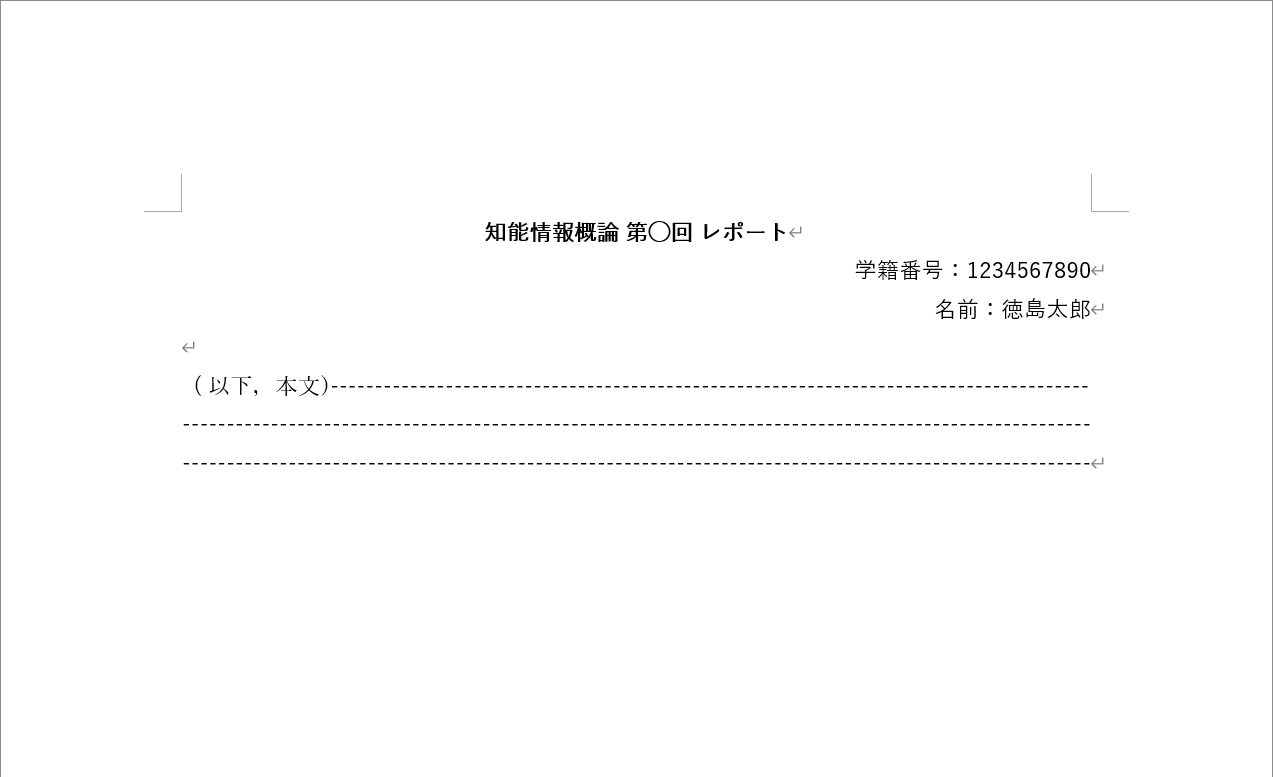
\includegraphics[width=10cm]{fig/title.png}
  \caption{レポート見出しの例}
  \label{fig:title}
\end{figure}

図\ref{fig:title}の例では,タイトルは太字にして,中央揃えにしています.(必ずそうしなければいけない,というわけではないです)
また,学籍番号と氏名は右揃えにしています.
好みや作成スタイルにもよりますが,タイトルを本文より少し大きめにすることもあります.

次に,フォントについてです.
レポートを作成する際には,フォントにも注意を払う必要があります.
基本的には,見出しにはゴシック体を,本文には明朝体を使用することが一般的です.
(ちなみに,この組み合わせは論文や報告書などで一般的に使用されるフォントの組み合わせです)
図\ref{fig:title}では,タイトルには遊ゴシック,本文には遊明朝を使用しています.

\subsection{図・表の挿入}
レポートには,図や表を挿入することがあります.
図や表を挿入する際には,図番号や表番号をつけることが一般的です.
このとき,注意することとして,図番号は図の下に,表番号は表の上に記載することが一般的です.
また,挿入した図や表については,必ず本文中で言及しておく必要があります.

\subsection{ページ番号}
レポートを作成する際には,必ずページ番号を挿入するようにしましょう.
ページ番号の挿入については,最後にやると忘れたまま提出してしまうことがあるので,レポート作成に取り掛かるタイミングで最初にやっておくことをおすすめします.
Wordでは,「挿入」タブから,「ページ番号」,「下部中央」という順番で選択するとページ番号を挿入することができます.

\subsection{参考文献}
レポートを作成する際には,外部の文献から本文や図を引用したりすることがあります.
その際には,必ず参考文献リストを作成し,本文中で引用した文献を明記する必要があります.
参考文献を適切に記述しないことは,重大なマナー違反であり,学術的な不正行為となります.

参考文献は,本文とは別に,レポートの最後に記載します.このとき,章番号はつけず,参考文献リストのみを記載します.
参考文献の書式には,様々なものがあります.
授業レポートであれば,参考文献のフォーマットについて指定されることは少ないですが,学会等に論文を投稿する際は,指定されることが多いです.
具体的なフォーマットについては,全国の大学付属図書館が公開している「論文の書き方」
\footnote{東京大学附属図書館:「レポート・論文作成支援」\url{https://www.lib.u-tokyo.ac.jp/ja/library/literacy/user-guide/campus/report}}
\footnote{京都大学桂図書館:「レポート・論文の書き方」\url{https://www.t.kyoto-u.ac.jp/lib/ja/support/tips/writing}}などを参考にしてください.

ウェブサイトの記事等を引用する場合は,発信されている情報が正確であるかどうかを確認することが重要です.
個人のブログではなく,できるだけ公的機関や企業等のページを参照するようにしましょう.
また,ウェブサイトは削除されたり,変更されたりすることがあるため,ウェブサイトを引用する際は,最終閲覧日を記載するようにしましょう.

\section{課題}
今週はプログラム課題はありません.余裕があれば来週のためにSVM(Support Vector Machine)など分類モデルについて調べておいてください.(レポートに記載する必要はありません.)
\subsection{調査課題}
以下に示す項目について調べてください.調べた内容と,参考文献を記載してください.なお,参考文献は,SIST02形式で記載してください.なお,SIST02については,独立行政法人科学技術振興機構「参考文献の役割と書き方\footnote{\url{https://warp.ndl.go.jp/info:ndljp/pid/12003258/jipsti.jst.go.jp/sist/pdf/SIST\_booklet2011.pdf}}」を参照してください.
\begin{itemize}
  \item 正規化と標準化
  \item 過学習
  \item 機械学習とAI,深層学習(ディープラーニング)の違い
  \item 孫引き
\end{itemize}

\begin{thebibliography}{99}
  \bibitem{leapmotion} Leap Motion Controller 2, \url{https://leap2.ultraleap.com/products/leap-motion-controller-2/}
  \bibitem{akubun} 随想舎: 文章入門 わかりやすい文章を書くために, \url{https://www.zuisousha.co.jp/bunsyou/} \\\\
  (閲覧日: すべて2024年6月22日)
\end{thebibliography}

\end{document}
